\chapter{Architecture Design Guidelines}

\section{Leading requirements}

The following list of leading requirements is meant to guide the creation and maintenance
of design guidelines and design decisions. The most important requirements are first
and foremost leading arguments in any comparison of alternatives. 

\begin{description}

	\item[Portability leads] We need the design tool to run equally well on all defined platforms
	and possibly platforms not (yet) defined. For that reason portability is a leading requirement.
	
	\item[Ease of use seconds] We need the design tool to assist in the design of \Noc and
	the development of verification tools with respect to \Noc designs. For that reason the design
	tool should facilitate these activities as much as possible. 
	
	\item[Maintainability third] The ease of maintenance was one of the primary requirements and
	as such should guide future design decisions. 
	
	\item[Performance follows] Under normal circumstances performance arguments should not lead.
	However, unacceptable performance will override all other considerations, because
	unacceptable performance disrupts use of the tool. 
	
	\item[Remark] What is acceptable performance is subjective. 
	
\end{description}

\paragraph{Example} When given a choice between alternatives with equal portability and 
ease of use consequences, the maintenance arguments should lead at the cost of performance 
provided the performance seems acceptable.

\section{High level design guidelines}

\begin{description}

	\item[C++ constructs lead] We strive to use C++ of the latest standard, currently C++ 2011.
	This implies the use of the C++ library including containers.
	
	\item[Boost] We use \boost as our goto library for portability. For mechanisms that would
	otherwise require platform dependent code we use \boost. Messaging, process control and
	interprocess communication is all directed through \boost.
	
	\item[fltk] We use the GUI library \fltk (pronounce ``\texttt{fulltick}'') for all GUI code.
	This takes care of most of the performance concerns for a graphical user interface.
	
	\item[OpenGL] Where we need extra drawing power we use \opengl or the \fltk \w{gl} extentions.
	This takes care of the remaining performance concerns that might exist.
	
\end{description}

\section{Observer pattern}

We use our own observer pattern as described in the \w{GoF}. 
Figure \ref{fig:observer-applied} the pattern applies the principle. 
Any object wanting to observe one of the subjects, needs to 
derive from \w{ConcreteObserver}.

\begin{center}
	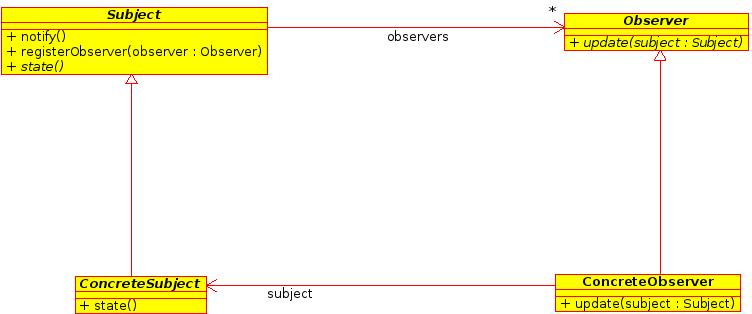
\includegraphics[width=.7\linewidth]{ObserverClassDiagram.jpeg}
	\captionof{figure}{Observer pattern as described in \w{GoF}}
	\label{fig:observer-pattern}
\end{center}

\begin{center}
	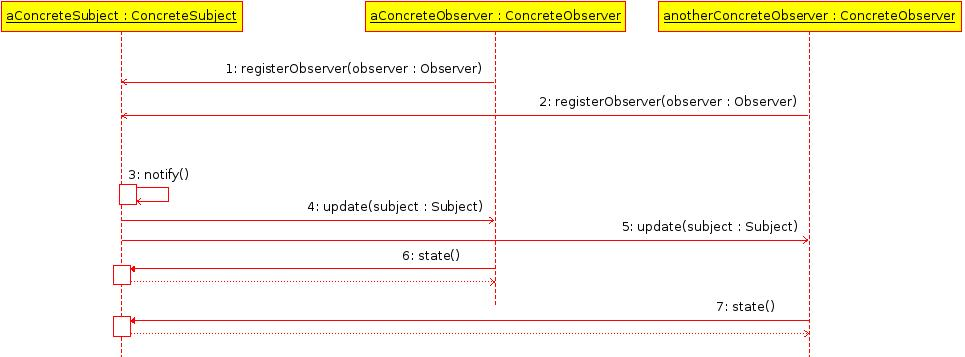
\includegraphics[width=.7\linewidth]{ObserverSequenceDiagram.jpeg}
	\captionof{figure}{Observer pattern applied}
	\label{fig:observer-applied}
\end{center}

